% Created by tikzDevice version 0.12.3.1 on 2022-05-11 22:31:02
% !TEX encoding = UTF-8 Unicode
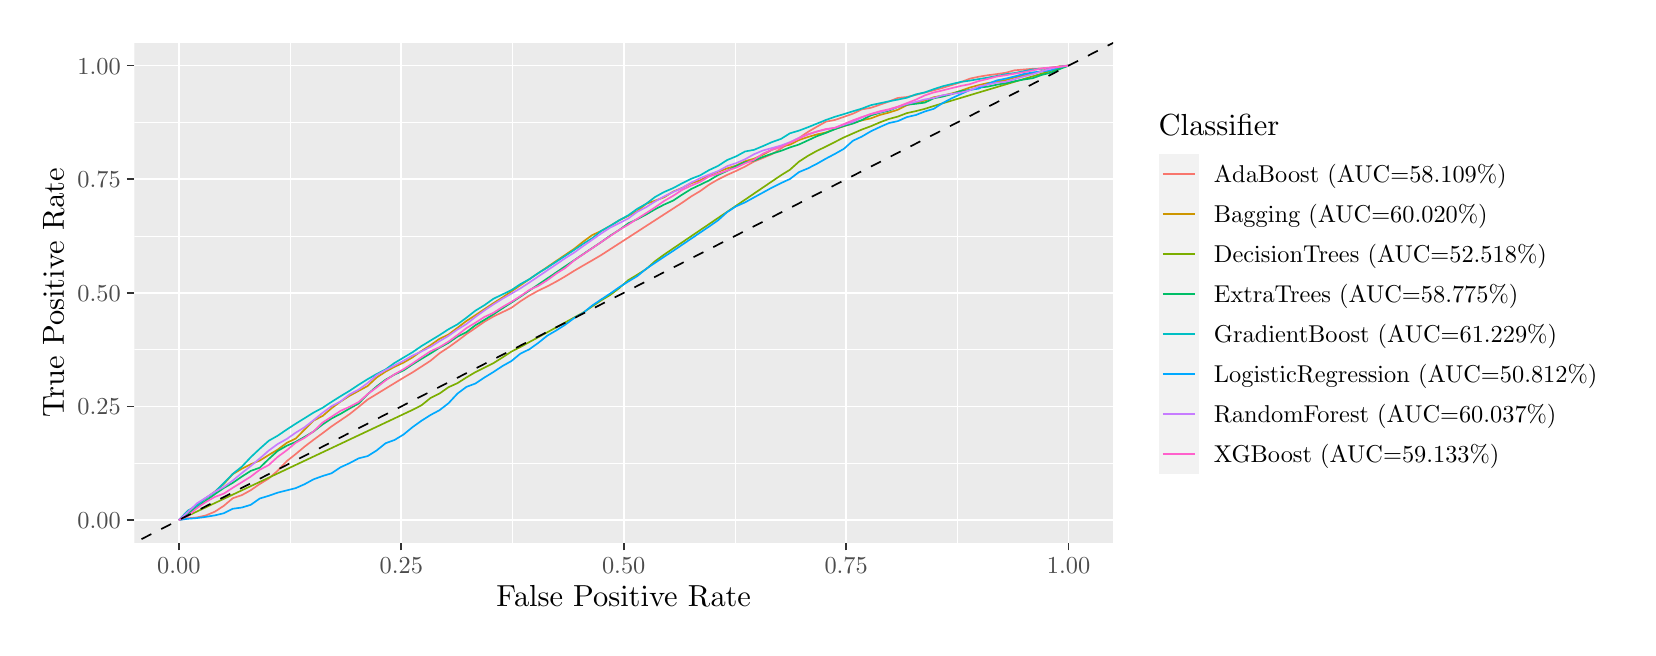
\begin{tikzpicture}[x=1pt,y=1pt]
\definecolor{fillColor}{RGB}{255,255,255}
\path[use as bounding box,fill=fillColor,fill opacity=0.00] (0,0) rectangle (578.16,216.81);
\begin{scope}
\path[clip] (  0.00,  0.00) rectangle (578.16,216.81);
\definecolor{drawColor}{RGB}{255,255,255}
\definecolor{fillColor}{RGB}{255,255,255}

\path[draw=drawColor,line width= 0.6pt,line join=round,line cap=round,fill=fillColor] (  0.00,  0.00) rectangle (578.16,216.81);
\end{scope}
\begin{scope}
\path[clip] ( 38.56, 30.69) rectangle (392.21,211.31);
\definecolor{fillColor}{gray}{0.92}

\path[fill=fillColor] ( 38.56, 30.69) rectangle (392.21,211.31);
\definecolor{drawColor}{RGB}{255,255,255}

\path[draw=drawColor,line width= 0.3pt,line join=round] ( 38.56, 59.42) --
	(392.21, 59.42);

\path[draw=drawColor,line width= 0.3pt,line join=round] ( 38.56,100.47) --
	(392.21,100.47);

\path[draw=drawColor,line width= 0.3pt,line join=round] ( 38.56,141.52) --
	(392.21,141.52);

\path[draw=drawColor,line width= 0.3pt,line join=round] ( 38.56,182.57) --
	(392.21,182.57);

\path[draw=drawColor,line width= 0.3pt,line join=round] ( 94.82, 30.69) --
	( 94.82,211.31);

\path[draw=drawColor,line width= 0.3pt,line join=round] (175.20, 30.69) --
	(175.20,211.31);

\path[draw=drawColor,line width= 0.3pt,line join=round] (255.57, 30.69) --
	(255.57,211.31);

\path[draw=drawColor,line width= 0.3pt,line join=round] (335.95, 30.69) --
	(335.95,211.31);

\path[draw=drawColor,line width= 0.6pt,line join=round] ( 38.56, 38.90) --
	(392.21, 38.90);

\path[draw=drawColor,line width= 0.6pt,line join=round] ( 38.56, 79.95) --
	(392.21, 79.95);

\path[draw=drawColor,line width= 0.6pt,line join=round] ( 38.56,121.00) --
	(392.21,121.00);

\path[draw=drawColor,line width= 0.6pt,line join=round] ( 38.56,162.05) --
	(392.21,162.05);

\path[draw=drawColor,line width= 0.6pt,line join=round] ( 38.56,203.10) --
	(392.21,203.10);

\path[draw=drawColor,line width= 0.6pt,line join=round] ( 54.63, 30.69) --
	( 54.63,211.31);

\path[draw=drawColor,line width= 0.6pt,line join=round] (135.01, 30.69) --
	(135.01,211.31);

\path[draw=drawColor,line width= 0.6pt,line join=round] (215.38, 30.69) --
	(215.38,211.31);

\path[draw=drawColor,line width= 0.6pt,line join=round] (295.76, 30.69) --
	(295.76,211.31);

\path[draw=drawColor,line width= 0.6pt,line join=round] (376.14, 30.69) --
	(376.14,211.31);
\definecolor{drawColor}{RGB}{248,118,109}

\path[draw=drawColor,line width= 0.6pt,line join=round] ( 54.63, 38.90) --
	( 57.88, 39.55) --
	( 61.13, 39.82) --
	( 64.37, 40.55) --
	( 67.62, 41.91) --
	( 70.87, 44.03) --
	( 74.12, 46.78) --
	( 77.36, 47.88) --
	( 80.61, 49.67) --
	( 83.86, 51.92) --
	( 87.11, 53.88) --
	( 90.35, 56.73) --
	( 93.60, 60.16) --
	( 96.85, 62.73) --
	(100.10, 65.45) --
	(103.34, 67.92) --
	(106.59, 70.29) --
	(109.84, 72.75) --
	(113.09, 74.95) --
	(116.33, 77.16) --
	(119.58, 79.76) --
	(122.83, 82.42) --
	(126.08, 84.40) --
	(129.32, 86.38) --
	(132.57, 88.36) --
	(135.82, 90.34) --
	(139.07, 92.25) --
	(142.31, 94.34) --
	(145.56, 96.45) --
	(148.81, 99.14) --
	(152.06,101.29) --
	(155.30,103.61) --
	(158.55,106.08) --
	(161.80,108.28) --
	(165.05,110.55) --
	(168.29,112.43) --
	(171.54,113.99) --
	(174.79,115.57) --
	(178.04,117.93) --
	(181.28,119.99) --
	(184.53,121.79) --
	(187.78,123.33) --
	(191.03,125.07) --
	(194.27,126.95) --
	(197.52,128.98) --
	(200.77,130.88) --
	(204.02,132.74) --
	(207.26,134.65) --
	(210.51,136.75) --
	(213.76,138.85) --
	(217.01,140.95) --
	(220.26,143.05) --
	(223.50,145.15) --
	(226.75,147.25) --
	(230.00,149.35) --
	(233.25,151.45) --
	(236.49,153.55) --
	(239.74,155.81) --
	(242.99,157.75) --
	(246.24,160.08) --
	(249.48,161.98) --
	(252.73,163.59) --
	(255.98,165.04) --
	(259.23,166.62) --
	(262.47,168.44) --
	(265.72,169.75) --
	(268.97,171.11) --
	(272.22,173.15) --
	(275.46,175.24) --
	(278.71,176.95) --
	(281.96,179.16) --
	(285.21,181.04) --
	(288.45,182.84) --
	(291.70,183.46) --
	(294.95,184.59) --
	(298.20,185.72) --
	(301.44,187.28) --
	(304.69,187.85) --
	(307.94,188.96) --
	(311.19,190.12) --
	(314.43,191.42) --
	(317.68,191.75) --
	(320.93,192.51) --
	(324.18,193.37) --
	(327.42,194.18) --
	(330.67,195.07) --
	(333.92,196.07) --
	(337.17,197.10) --
	(340.41,198.38) --
	(343.66,199.08) --
	(346.91,199.62) --
	(350.16,200.03) --
	(353.40,200.52) --
	(356.65,201.41) --
	(359.90,201.68) --
	(363.15,201.96) --
	(366.39,202.07) --
	(369.64,202.34) --
	(372.89,202.50) --
	(376.14,203.10);
\definecolor{drawColor}{RGB}{205,150,0}

\path[draw=drawColor,line width= 0.6pt,line join=round] ( 54.63, 38.90) --
	( 57.88, 41.67) --
	( 61.13, 44.41) --
	( 64.37, 46.77) --
	( 67.62, 49.13) --
	( 70.87, 51.92) --
	( 74.12, 55.49) --
	( 77.36, 57.42) --
	( 80.61, 59.07) --
	( 83.86, 60.37) --
	( 87.11, 62.41) --
	( 90.35, 64.34) --
	( 93.60, 66.77) --
	( 96.85, 68.33) --
	(100.10, 71.64) --
	(103.34, 74.84) --
	(106.59, 76.51) --
	(109.84, 79.32) --
	(113.09, 81.71) --
	(116.33, 83.79) --
	(119.58, 85.56) --
	(122.83, 87.32) --
	(126.08, 90.37) --
	(129.32, 92.51) --
	(132.57, 94.25) --
	(135.82, 95.78) --
	(139.07, 97.67) --
	(142.31,100.01) --
	(145.56,102.08) --
	(148.81,104.37) --
	(152.06,105.92) --
	(155.30,108.37) --
	(158.55,110.82) --
	(161.80,112.92) --
	(165.05,115.09) --
	(168.29,117.25) --
	(171.54,119.31) --
	(174.79,121.51) --
	(178.04,123.72) --
	(181.28,125.92) --
	(184.53,128.12) --
	(187.78,130.32) --
	(191.03,132.53) --
	(194.27,134.73) --
	(197.52,136.93) --
	(200.77,139.53) --
	(204.02,141.88) --
	(207.26,143.36) --
	(210.51,145.19) --
	(213.76,147.18) --
	(217.01,148.81) --
	(220.26,150.51) --
	(223.50,153.14) --
	(226.75,154.31) --
	(230.00,155.53) --
	(233.25,157.56) --
	(236.49,158.92) --
	(239.74,160.58) --
	(242.99,161.64) --
	(246.24,163.46) --
	(249.48,164.74) --
	(252.73,165.95) --
	(255.98,166.98) --
	(259.23,168.57) --
	(262.47,169.46) --
	(265.72,170.92) --
	(268.97,172.71) --
	(272.22,173.80) --
	(275.46,174.55) --
	(278.71,176.20) --
	(281.96,177.31) --
	(285.21,178.24) --
	(288.45,178.95) --
	(291.70,180.20) --
	(294.95,181.20) --
	(298.20,182.27) --
	(301.44,183.32) --
	(304.69,184.04) --
	(307.94,185.27) --
	(311.19,186.11) --
	(314.43,187.16) --
	(317.68,188.81) --
	(320.93,189.67) --
	(324.18,190.45) --
	(327.42,191.68) --
	(330.67,192.28) --
	(333.92,193.04) --
	(337.17,194.02) --
	(340.41,195.17) --
	(343.66,196.04) --
	(346.91,196.79) --
	(350.16,197.26) --
	(353.40,197.86) --
	(356.65,198.84) --
	(359.90,199.49) --
	(363.15,200.29) --
	(366.39,201.06) --
	(369.64,202.26) --
	(372.89,202.86) --
	(376.14,203.10);
\definecolor{drawColor}{RGB}{124,174,0}

\path[draw=drawColor,line width= 0.6pt,line join=round] ( 54.63, 38.90) --
	( 57.88, 40.43) --
	( 61.13, 41.96) --
	( 64.37, 43.49) --
	( 67.62, 45.02) --
	( 70.87, 46.55) --
	( 74.12, 48.08) --
	( 77.36, 49.61) --
	( 80.61, 51.14) --
	( 83.86, 52.67) --
	( 87.11, 54.20) --
	( 90.35, 55.73) --
	( 93.60, 57.27) --
	( 96.85, 58.80) --
	(100.10, 60.33) --
	(103.34, 61.86) --
	(106.59, 63.39) --
	(109.84, 64.92) --
	(113.09, 66.45) --
	(116.33, 67.98) --
	(119.58, 69.51) --
	(122.83, 71.04) --
	(126.08, 72.57) --
	(129.32, 74.10) --
	(132.57, 75.63) --
	(135.82, 77.17) --
	(139.07, 78.70) --
	(142.31, 80.36) --
	(145.56, 82.99) --
	(148.81, 84.60) --
	(152.06, 86.89) --
	(155.30, 88.35) --
	(158.55, 90.42) --
	(161.80, 92.35) --
	(165.05, 93.96) --
	(168.29, 95.58) --
	(171.54, 97.62) --
	(174.79, 99.75) --
	(178.04,101.40) --
	(181.28,103.21) --
	(184.53,104.96) --
	(187.78,106.74) --
	(191.03,108.52) --
	(194.27,110.31) --
	(197.52,112.10) --
	(200.77,113.89) --
	(204.02,116.10) --
	(207.26,118.28) --
	(210.51,120.23) --
	(213.76,122.70) --
	(217.01,125.58) --
	(220.26,127.53) --
	(223.50,129.58) --
	(226.75,132.46) --
	(230.00,134.82) --
	(233.25,137.03) --
	(236.49,139.23) --
	(239.74,141.44) --
	(242.99,143.64) --
	(246.24,145.84) --
	(249.48,148.05) --
	(252.73,150.25) --
	(255.98,152.46) --
	(259.23,154.66) --
	(262.47,156.87) --
	(265.72,159.07) --
	(268.97,161.28) --
	(272.22,163.48) --
	(275.46,165.48) --
	(278.71,168.40) --
	(281.96,170.50) --
	(285.21,172.31) --
	(288.45,173.84) --
	(291.70,175.50) --
	(294.95,177.15) --
	(298.20,178.59) --
	(301.44,180.00) --
	(304.69,181.20) --
	(307.94,182.59) --
	(311.19,183.81) --
	(314.43,184.69) --
	(317.68,185.93) --
	(320.93,186.65) --
	(324.18,187.48) --
	(327.42,188.51) --
	(330.67,189.49) --
	(333.92,190.46) --
	(337.17,191.43) --
	(340.41,192.40) --
	(343.66,193.38) --
	(346.91,194.35) --
	(350.16,195.32) --
	(353.40,196.29) --
	(356.65,197.27) --
	(359.90,198.24) --
	(363.15,199.21) --
	(366.39,200.18) --
	(369.64,201.16) --
	(372.89,202.13) --
	(376.14,203.10);
\definecolor{drawColor}{RGB}{0,190,103}

\path[draw=drawColor,line width= 0.6pt,line join=round] ( 54.63, 38.90) --
	( 57.88, 41.23) --
	( 61.13, 43.56) --
	( 64.37, 45.90) --
	( 67.62, 48.23) --
	( 70.87, 50.47) --
	( 74.12, 52.34) --
	( 77.36, 54.57) --
	( 80.61, 56.65) --
	( 83.86, 57.80) --
	( 87.11, 60.94) --
	( 90.35, 63.87) --
	( 93.60, 65.72) --
	( 96.85, 67.13) --
	(100.10, 68.97) --
	(103.34, 70.90) --
	(106.59, 73.45) --
	(109.84, 75.61) --
	(113.09, 77.29) --
	(116.33, 79.19) --
	(119.58, 80.98) --
	(122.83, 84.33) --
	(126.08, 87.16) --
	(129.32, 89.59) --
	(132.57, 91.46) --
	(135.82, 92.96) --
	(139.07, 95.12) --
	(142.31, 97.14) --
	(145.56, 99.09) --
	(148.81,101.15) --
	(152.06,102.93) --
	(155.30,105.16) --
	(158.55,106.79) --
	(161.80,109.29) --
	(165.05,111.23) --
	(168.29,113.21) --
	(171.54,115.37) --
	(174.79,117.44) --
	(178.04,119.60) --
	(181.28,121.80) --
	(184.53,124.00) --
	(187.78,126.20) --
	(191.03,128.40) --
	(194.27,130.60) --
	(197.52,132.80) --
	(200.77,135.00) --
	(204.02,137.20) --
	(207.26,139.35) --
	(210.51,141.66) --
	(213.76,143.71) --
	(217.01,146.09) --
	(220.26,147.58) --
	(223.50,149.31) --
	(226.75,151.20) --
	(230.00,152.89) --
	(233.25,154.34) --
	(236.49,156.47) --
	(239.74,158.49) --
	(242.99,160.04) --
	(246.24,161.61) --
	(249.48,163.56) --
	(252.73,165.05) --
	(255.98,166.82) --
	(259.23,168.18) --
	(262.47,168.78) --
	(265.72,170.12) --
	(268.97,171.29) --
	(272.22,172.29) --
	(275.46,173.54) --
	(278.71,174.59) --
	(281.96,176.09) --
	(285.21,177.60) --
	(288.45,178.78) --
	(291.70,180.12) --
	(294.95,181.30) --
	(298.20,182.15) --
	(301.44,183.43) --
	(304.69,185.11) --
	(307.94,186.05) --
	(311.19,186.82) --
	(314.43,188.16) --
	(317.68,188.98) --
	(320.93,189.30) --
	(324.18,189.73) --
	(327.42,191.28) --
	(330.67,191.91) --
	(333.92,192.79) --
	(337.17,193.89) --
	(340.41,194.30) --
	(343.66,195.13) --
	(346.91,195.49) --
	(350.16,196.20) --
	(353.40,196.75) --
	(356.65,197.45) --
	(359.90,198.06) --
	(363.15,198.54) --
	(366.39,199.72) --
	(369.64,200.53) --
	(372.89,201.83) --
	(376.14,203.10);
\definecolor{drawColor}{RGB}{0,191,196}

\path[draw=drawColor,line width= 0.6pt,line join=round] ( 54.63, 38.90) --
	( 57.88, 42.29) --
	( 61.13, 44.10) --
	( 64.37, 46.81) --
	( 67.62, 48.98) --
	( 70.87, 52.25) --
	( 74.12, 55.59) --
	( 77.36, 58.15) --
	( 80.61, 61.59) --
	( 83.86, 64.65) --
	( 87.11, 67.54) --
	( 90.35, 69.37) --
	( 93.60, 71.59) --
	( 96.85, 73.70) --
	(100.10, 75.71) --
	(103.34, 77.74) --
	(106.59, 79.46) --
	(109.84, 81.61) --
	(113.09, 83.65) --
	(116.33, 85.60) --
	(119.58, 87.76) --
	(122.83, 89.79) --
	(126.08, 91.65) --
	(129.32, 93.30) --
	(132.57, 95.66) --
	(135.82, 97.60) --
	(139.07, 99.53) --
	(142.31,101.76) --
	(145.56,103.74) --
	(148.81,105.71) --
	(152.06,107.83) --
	(155.30,109.60) --
	(158.55,112.00) --
	(161.80,114.56) --
	(165.05,116.53) --
	(168.29,118.84) --
	(171.54,120.41) --
	(174.79,121.98) --
	(178.04,124.15) --
	(181.28,125.91) --
	(184.53,128.15) --
	(187.78,130.12) --
	(191.03,132.27) --
	(194.27,134.36) --
	(197.52,136.54) --
	(200.77,138.74) --
	(204.02,140.75) --
	(207.26,143.38) --
	(210.51,145.21) --
	(213.76,147.22) --
	(217.01,149.01) --
	(220.26,151.34) --
	(223.50,153.18) --
	(226.75,155.65) --
	(230.00,157.44) --
	(233.25,158.84) --
	(236.49,160.58) --
	(239.74,162.20) --
	(242.99,163.45) --
	(246.24,165.35) --
	(249.48,166.86) --
	(252.73,168.97) --
	(255.98,170.30) --
	(259.23,172.07) --
	(262.47,172.67) --
	(265.72,174.03) --
	(268.97,175.47) --
	(272.22,176.62) --
	(275.46,178.65) --
	(278.71,179.61) --
	(281.96,180.83) --
	(285.21,182.15) --
	(288.45,183.46) --
	(291.70,184.61) --
	(294.95,185.58) --
	(298.20,186.60) --
	(301.44,187.57) --
	(304.69,188.81) --
	(307.94,189.50) --
	(311.19,190.19) --
	(314.43,190.82) --
	(317.68,191.48) --
	(320.93,192.71) --
	(324.18,193.42) --
	(327.42,194.59) --
	(330.67,195.65) --
	(333.92,196.44) --
	(337.17,197.21) --
	(340.41,197.67) --
	(343.66,198.23) --
	(346.91,198.75) --
	(350.16,199.35) --
	(353.40,200.00) --
	(356.65,200.41) --
	(359.90,201.06) --
	(363.15,201.69) --
	(366.39,201.96) --
	(369.64,202.31) --
	(372.89,202.47) --
	(376.14,203.10);
\definecolor{drawColor}{RGB}{0,169,255}

\path[draw=drawColor,line width= 0.6pt,line join=round] ( 54.63, 38.90) --
	( 57.88, 39.36) --
	( 61.13, 39.60) --
	( 64.37, 40.04) --
	( 67.62, 40.58) --
	( 70.87, 41.34) --
	( 74.12, 42.97) --
	( 77.36, 43.41) --
	( 80.61, 44.39) --
	( 83.86, 46.67) --
	( 87.11, 47.65) --
	( 90.35, 48.79) --
	( 93.60, 49.61) --
	( 96.85, 50.42) --
	(100.10, 51.86) --
	(103.34, 53.63) --
	(106.59, 54.80) --
	(109.84, 55.81) --
	(113.09, 57.98) --
	(116.33, 59.45) --
	(119.58, 61.18) --
	(122.83, 61.99) --
	(126.08, 64.02) --
	(129.32, 66.64) --
	(132.57, 67.83) --
	(135.82, 69.79) --
	(139.07, 72.46) --
	(142.31, 74.78) --
	(145.56, 76.84) --
	(148.81, 78.58) --
	(152.06, 81.09) --
	(155.30, 84.58) --
	(158.55, 87.01) --
	(161.80, 88.23) --
	(165.05, 90.40) --
	(168.29, 92.38) --
	(171.54, 94.52) --
	(174.79, 96.34) --
	(178.04, 99.02) --
	(181.28,100.59) --
	(184.53,102.92) --
	(187.78,105.53) --
	(191.03,107.42) --
	(194.27,109.48) --
	(197.52,111.90) --
	(200.77,113.77) --
	(204.02,116.44) --
	(207.26,118.62) --
	(210.51,120.75) --
	(213.76,123.03) --
	(217.01,125.06) --
	(220.26,127.01) --
	(223.50,129.67) --
	(226.75,131.87) --
	(230.00,134.03) --
	(233.25,136.15) --
	(236.49,138.35) --
	(239.74,140.55) --
	(242.99,142.75) --
	(246.24,144.95) --
	(249.48,147.21) --
	(252.73,150.14) --
	(255.98,152.25) --
	(259.23,153.68) --
	(262.47,155.47) --
	(265.72,157.25) --
	(268.97,159.03) --
	(272.22,160.65) --
	(275.46,162.13) --
	(278.71,164.62) --
	(281.96,165.97) --
	(285.21,167.64) --
	(288.45,169.49) --
	(291.70,171.20) --
	(294.95,173.04) --
	(298.20,175.94) --
	(301.44,177.46) --
	(304.69,179.37) --
	(307.94,180.90) --
	(311.19,182.33) --
	(314.43,183.04) --
	(317.68,184.49) --
	(320.93,185.24) --
	(324.18,186.52) --
	(327.42,187.49) --
	(330.67,189.59) --
	(333.92,191.30) --
	(337.17,192.80) --
	(340.41,194.29) --
	(343.66,194.78) --
	(346.91,196.49) --
	(350.16,197.74) --
	(353.40,198.40) --
	(356.65,199.19) --
	(359.90,200.05) --
	(363.15,200.63) --
	(366.39,200.98) --
	(369.64,201.39) --
	(372.89,202.64) --
	(376.14,203.10);
\definecolor{drawColor}{RGB}{199,124,255}

\path[draw=drawColor,line width= 0.6pt,line join=round] ( 54.63, 38.90) --
	( 57.88, 41.74) --
	( 61.13, 44.90) --
	( 64.37, 46.96) --
	( 67.62, 49.07) --
	( 70.87, 50.84) --
	( 74.12, 53.18) --
	( 77.36, 55.85) --
	( 80.61, 58.40) --
	( 83.86, 61.14) --
	( 87.11, 63.99) --
	( 90.35, 66.36) --
	( 93.60, 68.17) --
	( 96.85, 70.45) --
	(100.10, 72.45) --
	(103.34, 75.00) --
	(106.59, 77.66) --
	(109.84, 80.06) --
	(113.09, 81.77) --
	(116.33, 84.32) --
	(119.58, 86.02) --
	(122.83, 88.38) --
	(126.08, 91.24) --
	(129.32, 93.06) --
	(132.57, 94.77) --
	(135.82, 96.45) --
	(139.07, 98.33) --
	(142.31, 99.82) --
	(145.56,101.45) --
	(148.81,103.53) --
	(152.06,105.44) --
	(155.30,107.74) --
	(158.55,109.73) --
	(161.80,112.29) --
	(165.05,114.63) --
	(168.29,116.80) --
	(171.54,118.83) --
	(174.79,120.70) --
	(178.04,122.62) --
	(181.28,124.72) --
	(184.53,126.92) --
	(187.78,129.12) --
	(191.03,131.32) --
	(194.27,133.52) --
	(197.52,135.56) --
	(200.77,137.93) --
	(204.02,140.19) --
	(207.26,142.45) --
	(210.51,144.58) --
	(213.76,146.17) --
	(217.01,147.85) --
	(220.26,150.27) --
	(223.50,151.96) --
	(226.75,154.03) --
	(230.00,155.85) --
	(233.25,157.42) --
	(236.49,158.86) --
	(239.74,160.83) --
	(242.99,162.42) --
	(246.24,163.72) --
	(249.48,164.97) --
	(252.73,166.76) --
	(255.98,167.86) --
	(259.23,169.26) --
	(262.47,171.08) --
	(265.72,172.44) --
	(268.97,173.32) --
	(272.22,174.22) --
	(275.46,175.45) --
	(278.71,176.99) --
	(281.96,178.19) --
	(285.21,179.25) --
	(288.45,180.02) --
	(291.70,180.62) --
	(294.95,181.70) --
	(298.20,182.77) --
	(301.44,184.38) --
	(304.69,185.59) --
	(307.94,186.26) --
	(311.19,187.10) --
	(314.43,188.13) --
	(317.68,189.19) --
	(320.93,190.00) --
	(324.18,190.88) --
	(327.42,191.41) --
	(330.67,192.38) --
	(333.92,192.87) --
	(337.17,193.33) --
	(340.41,194.15) --
	(343.66,195.57) --
	(346.91,196.23) --
	(350.16,196.92) --
	(353.40,197.25) --
	(356.65,198.18) --
	(359.90,199.16) --
	(363.15,199.98) --
	(366.39,201.05) --
	(369.64,202.00) --
	(372.89,202.72) --
	(376.14,203.10);
\definecolor{drawColor}{RGB}{255,97,204}

\path[draw=drawColor,line width= 0.6pt,line join=round] ( 54.63, 38.90) --
	( 57.88, 40.34) --
	( 61.13, 43.16) --
	( 64.37, 45.39) --
	( 67.62, 47.24) --
	( 70.87, 48.44) --
	( 74.12, 50.56) --
	( 77.36, 52.55) --
	( 80.61, 54.58) --
	( 83.86, 57.05) --
	( 87.11, 58.77) --
	( 90.35, 61.71) --
	( 93.60, 64.09) --
	( 96.85, 66.81) --
	(100.10, 68.63) --
	(103.34, 70.94) --
	(106.59, 74.14) --
	(109.84, 76.24) --
	(113.09, 78.37) --
	(116.33, 79.82) --
	(119.58, 81.53) --
	(122.83, 84.38) --
	(126.08, 86.78) --
	(129.32, 89.35) --
	(132.57, 91.57) --
	(135.82, 93.39) --
	(139.07, 95.48) --
	(142.31, 97.72) --
	(145.56, 99.87) --
	(148.81,101.37) --
	(152.06,103.36) --
	(155.30,105.72) --
	(158.55,108.25) --
	(161.80,110.19) --
	(165.05,112.29) --
	(168.29,113.77) --
	(171.54,115.86) --
	(174.79,117.73) --
	(178.04,119.79) --
	(181.28,122.04) --
	(184.53,123.51) --
	(187.78,125.56) --
	(191.03,127.96) --
	(194.27,129.98) --
	(197.52,132.74) --
	(200.77,134.93) --
	(204.02,137.13) --
	(207.26,139.33) --
	(210.51,141.53) --
	(213.76,143.73) --
	(217.01,145.63) --
	(220.26,147.76) --
	(223.50,149.80) --
	(226.75,151.92) --
	(230.00,154.20) --
	(233.25,156.06) --
	(236.49,158.19) --
	(239.74,159.73) --
	(242.99,161.09) --
	(246.24,163.03) --
	(249.48,164.03) --
	(252.73,165.15) --
	(255.98,166.23) --
	(259.23,167.79) --
	(262.47,169.08) --
	(265.72,171.31) --
	(268.97,172.71) --
	(272.22,173.71) --
	(275.46,175.24) --
	(278.71,176.72) --
	(281.96,178.31) --
	(285.21,179.31) --
	(288.45,180.18) --
	(291.70,180.64) --
	(294.95,181.99) --
	(298.20,183.33) --
	(301.44,184.52) --
	(304.69,185.62) --
	(307.94,186.62) --
	(311.19,187.32) --
	(314.43,188.27) --
	(317.68,189.54) --
	(320.93,190.79) --
	(324.18,192.35) --
	(327.42,193.40) --
	(330.67,194.15) --
	(333.92,194.97) --
	(337.17,195.76) --
	(340.41,196.38) --
	(343.66,197.50) --
	(346.91,198.29) --
	(350.16,199.14) --
	(353.40,199.62) --
	(356.65,200.19) --
	(359.90,200.71) --
	(363.15,201.36) --
	(366.39,202.09) --
	(369.64,202.45) --
	(372.89,202.64) --
	(376.14,203.10);
\definecolor{drawColor}{RGB}{0,0,0}

\path[draw=drawColor,line width= 0.6pt,dash pattern=on 4pt off 4pt ,line join=round] (-315.10,-149.94) -- (745.87,391.93);
\end{scope}
\begin{scope}
\path[clip] (  0.00,  0.00) rectangle (578.16,216.81);
\definecolor{drawColor}{gray}{0.30}

\node[text=drawColor,anchor=base east,inner sep=0pt, outer sep=0pt, scale=  0.88] at ( 33.61, 35.87) {0.00};

\node[text=drawColor,anchor=base east,inner sep=0pt, outer sep=0pt, scale=  0.88] at ( 33.61, 76.92) {0.25};

\node[text=drawColor,anchor=base east,inner sep=0pt, outer sep=0pt, scale=  0.88] at ( 33.61,117.97) {0.50};

\node[text=drawColor,anchor=base east,inner sep=0pt, outer sep=0pt, scale=  0.88] at ( 33.61,159.02) {0.75};

\node[text=drawColor,anchor=base east,inner sep=0pt, outer sep=0pt, scale=  0.88] at ( 33.61,200.07) {1.00};
\end{scope}
\begin{scope}
\path[clip] (  0.00,  0.00) rectangle (578.16,216.81);
\definecolor{drawColor}{gray}{0.20}

\path[draw=drawColor,line width= 0.6pt,line join=round] ( 35.81, 38.90) --
	( 38.56, 38.90);

\path[draw=drawColor,line width= 0.6pt,line join=round] ( 35.81, 79.95) --
	( 38.56, 79.95);

\path[draw=drawColor,line width= 0.6pt,line join=round] ( 35.81,121.00) --
	( 38.56,121.00);

\path[draw=drawColor,line width= 0.6pt,line join=round] ( 35.81,162.05) --
	( 38.56,162.05);

\path[draw=drawColor,line width= 0.6pt,line join=round] ( 35.81,203.10) --
	( 38.56,203.10);
\end{scope}
\begin{scope}
\path[clip] (  0.00,  0.00) rectangle (578.16,216.81);
\definecolor{drawColor}{gray}{0.20}

\path[draw=drawColor,line width= 0.6pt,line join=round] ( 54.63, 27.94) --
	( 54.63, 30.69);

\path[draw=drawColor,line width= 0.6pt,line join=round] (135.01, 27.94) --
	(135.01, 30.69);

\path[draw=drawColor,line width= 0.6pt,line join=round] (215.38, 27.94) --
	(215.38, 30.69);

\path[draw=drawColor,line width= 0.6pt,line join=round] (295.76, 27.94) --
	(295.76, 30.69);

\path[draw=drawColor,line width= 0.6pt,line join=round] (376.14, 27.94) --
	(376.14, 30.69);
\end{scope}
\begin{scope}
\path[clip] (  0.00,  0.00) rectangle (578.16,216.81);
\definecolor{drawColor}{gray}{0.30}

\node[text=drawColor,anchor=base,inner sep=0pt, outer sep=0pt, scale=  0.88] at ( 54.63, 19.68) {0.00};

\node[text=drawColor,anchor=base,inner sep=0pt, outer sep=0pt, scale=  0.88] at (135.01, 19.68) {0.25};

\node[text=drawColor,anchor=base,inner sep=0pt, outer sep=0pt, scale=  0.88] at (215.38, 19.68) {0.50};

\node[text=drawColor,anchor=base,inner sep=0pt, outer sep=0pt, scale=  0.88] at (295.76, 19.68) {0.75};

\node[text=drawColor,anchor=base,inner sep=0pt, outer sep=0pt, scale=  0.88] at (376.14, 19.68) {1.00};
\end{scope}
\begin{scope}
\path[clip] (  0.00,  0.00) rectangle (578.16,216.81);
\definecolor{drawColor}{RGB}{0,0,0}

\node[text=drawColor,anchor=base,inner sep=0pt, outer sep=0pt, scale=  1.10] at (215.38,  7.64) {False Positive Rate};
\end{scope}
\begin{scope}
\path[clip] (  0.00,  0.00) rectangle (578.16,216.81);
\definecolor{drawColor}{RGB}{0,0,0}

\node[text=drawColor,rotate= 90.00,anchor=base,inner sep=0pt, outer sep=0pt, scale=  1.10] at ( 13.08,121.00) {True Positive Rate};
\end{scope}
\begin{scope}
\path[clip] (  0.00,  0.00) rectangle (578.16,216.81);
\definecolor{fillColor}{RGB}{255,255,255}

\path[fill=fillColor] (403.21, 50.07) rectangle (572.66,191.92);
\end{scope}
\begin{scope}
\path[clip] (  0.00,  0.00) rectangle (578.16,216.81);
\definecolor{drawColor}{RGB}{0,0,0}

\node[text=drawColor,anchor=base west,inner sep=0pt, outer sep=0pt, scale=  1.10] at (408.71,177.78) {Classifier};
\end{scope}
\begin{scope}
\path[clip] (  0.00,  0.00) rectangle (578.16,216.81);
\definecolor{fillColor}{gray}{0.95}

\path[fill=fillColor] (408.71,156.75) rectangle (423.17,171.21);
\end{scope}
\begin{scope}
\path[clip] (  0.00,  0.00) rectangle (578.16,216.81);
\definecolor{drawColor}{RGB}{248,118,109}

\path[draw=drawColor,line width= 0.6pt,line join=round] (410.16,163.98) -- (421.72,163.98);
\end{scope}
\begin{scope}
\path[clip] (  0.00,  0.00) rectangle (578.16,216.81);
\definecolor{fillColor}{gray}{0.95}

\path[fill=fillColor] (408.71,142.30) rectangle (423.17,156.75);
\end{scope}
\begin{scope}
\path[clip] (  0.00,  0.00) rectangle (578.16,216.81);
\definecolor{drawColor}{RGB}{205,150,0}

\path[draw=drawColor,line width= 0.6pt,line join=round] (410.16,149.53) -- (421.72,149.53);
\end{scope}
\begin{scope}
\path[clip] (  0.00,  0.00) rectangle (578.16,216.81);
\definecolor{fillColor}{gray}{0.95}

\path[fill=fillColor] (408.71,127.84) rectangle (423.17,142.30);
\end{scope}
\begin{scope}
\path[clip] (  0.00,  0.00) rectangle (578.16,216.81);
\definecolor{drawColor}{RGB}{124,174,0}

\path[draw=drawColor,line width= 0.6pt,line join=round] (410.16,135.07) -- (421.72,135.07);
\end{scope}
\begin{scope}
\path[clip] (  0.00,  0.00) rectangle (578.16,216.81);
\definecolor{fillColor}{gray}{0.95}

\path[fill=fillColor] (408.71,113.39) rectangle (423.17,127.84);
\end{scope}
\begin{scope}
\path[clip] (  0.00,  0.00) rectangle (578.16,216.81);
\definecolor{drawColor}{RGB}{0,190,103}

\path[draw=drawColor,line width= 0.6pt,line join=round] (410.16,120.62) -- (421.72,120.62);
\end{scope}
\begin{scope}
\path[clip] (  0.00,  0.00) rectangle (578.16,216.81);
\definecolor{fillColor}{gray}{0.95}

\path[fill=fillColor] (408.71, 98.94) rectangle (423.17,113.39);
\end{scope}
\begin{scope}
\path[clip] (  0.00,  0.00) rectangle (578.16,216.81);
\definecolor{drawColor}{RGB}{0,191,196}

\path[draw=drawColor,line width= 0.6pt,line join=round] (410.16,106.16) -- (421.72,106.16);
\end{scope}
\begin{scope}
\path[clip] (  0.00,  0.00) rectangle (578.16,216.81);
\definecolor{fillColor}{gray}{0.95}

\path[fill=fillColor] (408.71, 84.48) rectangle (423.17, 98.94);
\end{scope}
\begin{scope}
\path[clip] (  0.00,  0.00) rectangle (578.16,216.81);
\definecolor{drawColor}{RGB}{0,169,255}

\path[draw=drawColor,line width= 0.6pt,line join=round] (410.16, 91.71) -- (421.72, 91.71);
\end{scope}
\begin{scope}
\path[clip] (  0.00,  0.00) rectangle (578.16,216.81);
\definecolor{fillColor}{gray}{0.95}

\path[fill=fillColor] (408.71, 70.03) rectangle (423.17, 84.48);
\end{scope}
\begin{scope}
\path[clip] (  0.00,  0.00) rectangle (578.16,216.81);
\definecolor{drawColor}{RGB}{199,124,255}

\path[draw=drawColor,line width= 0.6pt,line join=round] (410.16, 77.26) -- (421.72, 77.26);
\end{scope}
\begin{scope}
\path[clip] (  0.00,  0.00) rectangle (578.16,216.81);
\definecolor{fillColor}{gray}{0.95}

\path[fill=fillColor] (408.71, 55.57) rectangle (423.17, 70.03);
\end{scope}
\begin{scope}
\path[clip] (  0.00,  0.00) rectangle (578.16,216.81);
\definecolor{drawColor}{RGB}{255,97,204}

\path[draw=drawColor,line width= 0.6pt,line join=round] (410.16, 62.80) -- (421.72, 62.80);
\end{scope}
\begin{scope}
\path[clip] (  0.00,  0.00) rectangle (578.16,216.81);
\definecolor{drawColor}{RGB}{0,0,0}

\node[text=drawColor,anchor=base west,inner sep=0pt, outer sep=0pt, scale=  0.88] at (428.67,160.95) {AdaBoost (AUC=58.109\%)};
\end{scope}
\begin{scope}
\path[clip] (  0.00,  0.00) rectangle (578.16,216.81);
\definecolor{drawColor}{RGB}{0,0,0}

\node[text=drawColor,anchor=base west,inner sep=0pt, outer sep=0pt, scale=  0.88] at (428.67,146.50) {Bagging (AUC=60.020\%)};
\end{scope}
\begin{scope}
\path[clip] (  0.00,  0.00) rectangle (578.16,216.81);
\definecolor{drawColor}{RGB}{0,0,0}

\node[text=drawColor,anchor=base west,inner sep=0pt, outer sep=0pt, scale=  0.88] at (428.67,132.04) {DecisionTrees (AUC=52.518\%)};
\end{scope}
\begin{scope}
\path[clip] (  0.00,  0.00) rectangle (578.16,216.81);
\definecolor{drawColor}{RGB}{0,0,0}

\node[text=drawColor,anchor=base west,inner sep=0pt, outer sep=0pt, scale=  0.88] at (428.67,117.59) {ExtraTrees (AUC=58.775\%)};
\end{scope}
\begin{scope}
\path[clip] (  0.00,  0.00) rectangle (578.16,216.81);
\definecolor{drawColor}{RGB}{0,0,0}

\node[text=drawColor,anchor=base west,inner sep=0pt, outer sep=0pt, scale=  0.88] at (428.67,103.13) {GradientBoost (AUC=61.229\%)};
\end{scope}
\begin{scope}
\path[clip] (  0.00,  0.00) rectangle (578.16,216.81);
\definecolor{drawColor}{RGB}{0,0,0}

\node[text=drawColor,anchor=base west,inner sep=0pt, outer sep=0pt, scale=  0.88] at (428.67, 88.68) {LogisticRegression (AUC=50.812\%)};
\end{scope}
\begin{scope}
\path[clip] (  0.00,  0.00) rectangle (578.16,216.81);
\definecolor{drawColor}{RGB}{0,0,0}

\node[text=drawColor,anchor=base west,inner sep=0pt, outer sep=0pt, scale=  0.88] at (428.67, 74.23) {RandomForest (AUC=60.037\%)};
\end{scope}
\begin{scope}
\path[clip] (  0.00,  0.00) rectangle (578.16,216.81);
\definecolor{drawColor}{RGB}{0,0,0}

\node[text=drawColor,anchor=base west,inner sep=0pt, outer sep=0pt, scale=  0.88] at (428.67, 59.77) {XGBoost (AUC=59.133\%)};
\end{scope}
\end{tikzpicture}
